\documentclass[professionalfonts, aspectratio=169]{beamer}
\usepackage{newtxtext,newtxmath}
\usepackage[utf8]{inputenc}
\usepackage[russian]{babel}
\usepackage[T1]{fontenc} 
\usepackage{graphicx} 
\usepackage{bibentry} 
\usepackage{txfonts}
\setbeamertemplate{caption}[numbered]
\usepackage{caption}
\usepackage[alf]{abntex2cite}	
\usenavigationsymbolstemplate{}
\usepackage{helvet}
% Theme choice:
\usetheme{Boadilla}

\definecolor{UniBlue}{RGB}{32,64,154}
\definecolor{UniOrange}{cmyk}{0,50,100,0}

% Define as cores 
\setbeamercolor{title}{fg=UniBlue}
\setbeamercolor{author}{fg=UniBlue}
\setbeamercolor{institute}{fg=UniBlue}
\setbeamercolor{curso}{fg=UniBlue}
\setbeamercolor{frametitle}{fg=UniBlue}
\setbeamercolor{structure}{fg=UniBlue}
\setbeamercolor{normal text}{fg=black}
\usebeamercolor[fg]{normal text}
\setbeamercolor{enumerate}{fg=black}
\setbeamercolor{itemize}{fg=black}
\setbeamercolor{section in toc}{fg=black}
\setbeamercolor{subsection in toc}{fg=black}

% size*={<font size>}{<baseline skip>}
\setbeamerfont{title}{size=\fontsize{12pt}{8pt}}
\setbeamerfont{author}{size=\fontsize{16pt}{8pt}}
\setbeamerfont{institute}{size=\fontsize{16pt}{0pt}}
\setbeamerfont{curso}{size=\fontsize{14pt}{0pt}}

\addtobeamertemplate{institute}{\vspace*{20\baselineskip}}{}


\setbeamerfont{date}{size=\fontsize{8pt}{0pt}}

\setbeamerfont{frametitle}{size=\fontsize{16pt}{8pt}}
\addtobeamertemplate{frametitle}{\vspace*{1\baselineskip}}{}

\setbeamerfont{normal text}{size=\fontsize{10pt}{8pt}}
\setbeamerfont{enumerate}{size=\fontsize{10pt}{8pt}}
\setbeamerfont{itemize}{size=\fontsize{10pt}{8pt}}
\setbeamerfont{section in toc}{size=\fontsize{10pt}{8pt}}
\setbeamerfont{subsection in toc}{size=\fontsize{8pt}{8pt}}

\setbeamertemplate{title page}
{
    \vbox{}
    \vfill
    \begingroup
        \centering
        %-----------------institute
        \begin{beamercolorbox}[sep=8pt,right]{institute}
            \usebeamerfont{institute}\insertinstitute
        \end{beamercolorbox}
        %-----------------title
        \begin{beamercolorbox}[sep=8pt,right]{title}
            \usebeamerfont{title}\inserttitle\par%
        \end{beamercolorbox}%
    \endgroup
    \vfill
}

\title{Презентация в ЛаТех}
\author{Сиразитдинова Зарема}
\institute{Генетический алгоритм}

\newcommand*\oldmacro{}%
\let\oldmacro\insertshorttitle%
\renewcommand*\insertshorttitle{%
  \oldmacro\hfill%
  \insertframenumber\,/\,\inserttotalframenumber}

\logo{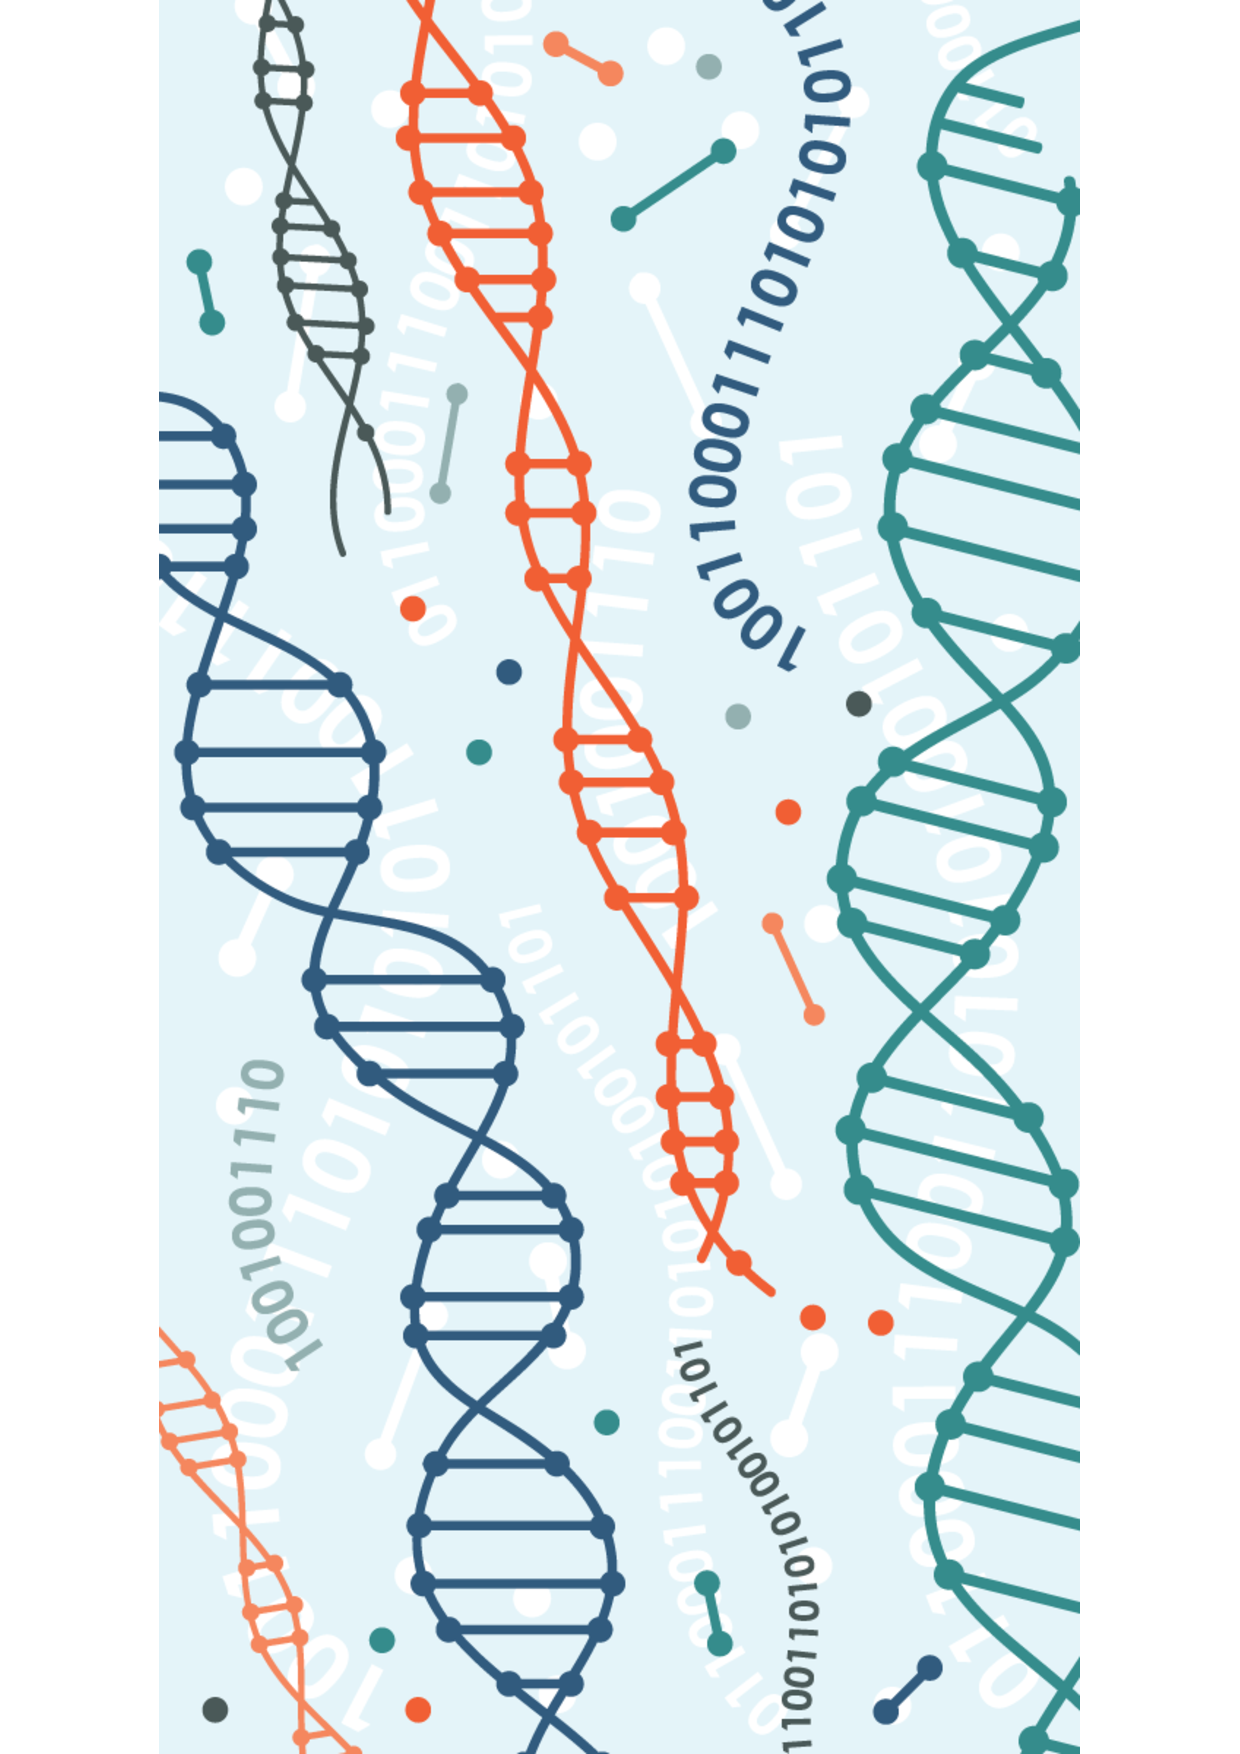
\includegraphics[height=1cm]{гены.pdf}}
\begin{document}
\def\beamer@andinst{\\[5em]}
\frame{\titlepage}
\section*{Содержание}
\begin{frame}{Содержание}
	\tableofcontents[]
\end{frame}
\section{Введение}
\begin{frame}[fragile=singleslide]{\insertsectionhead}
  \framesubtitle{\insertsubsectionhead}
В данном проекте рассматривается возможность создания компьютерного приложения, способного самостоятельно находить решение задач на построение с помощью циркуля и линейки в пространстве.  Разработка данного приложения опирается на так называемый генетический алгоритм, который впервые был применен в 1954 году Нильсом Баричелли на компьютере.
\begin{figure}
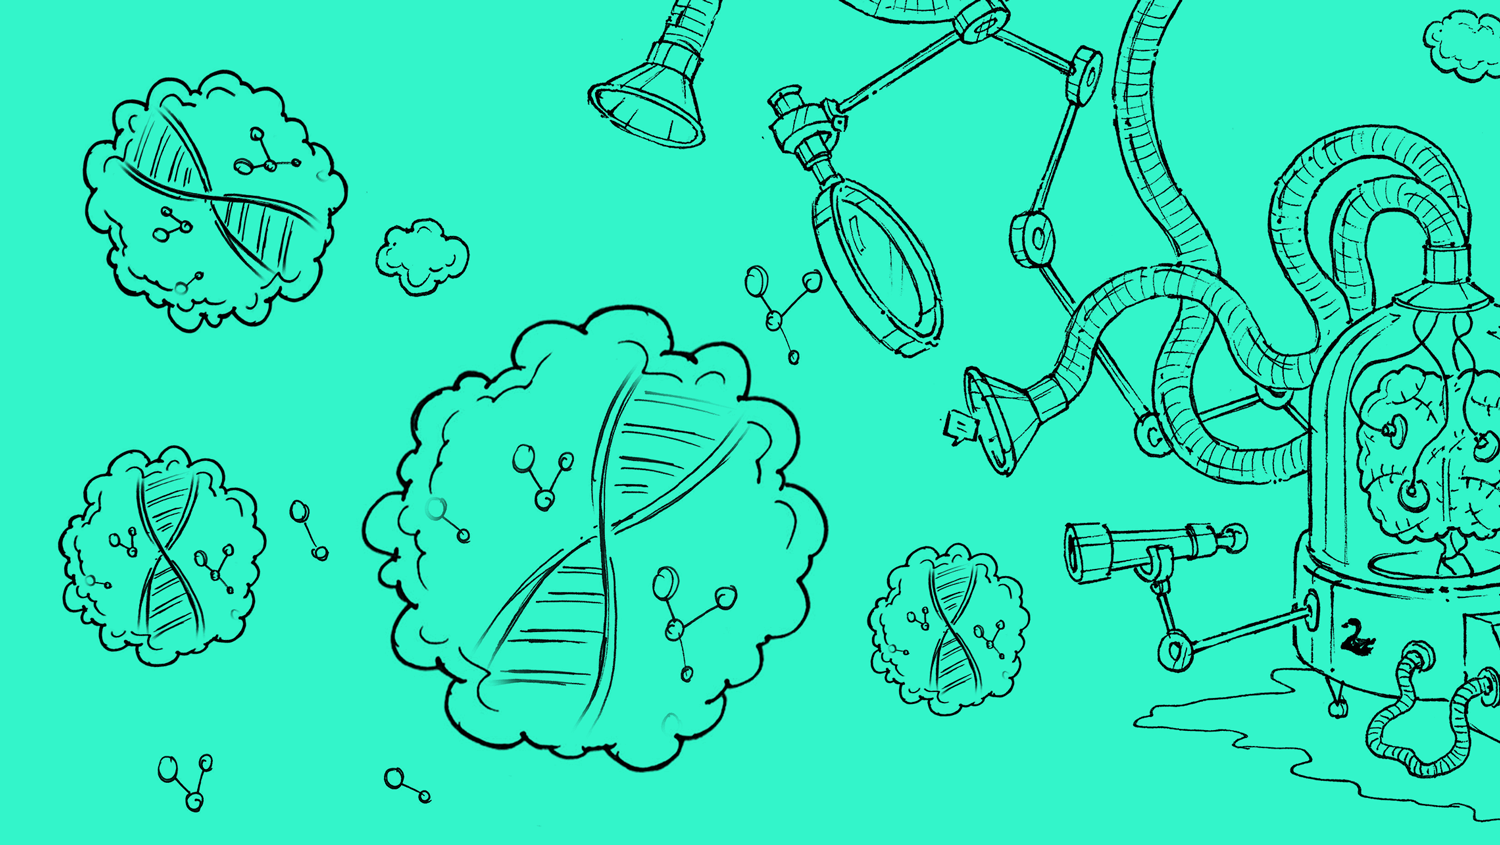
\includegraphics[width=0.5\textwidth]{введение.png} 
\caption{\label{fig:1}Введение}
\end{figure}
\end{frame}

\section{Барицентрические координаты}
\begin{frame}{Барицентрические координаты}
Еще одной важной теоремой является правило рычага для двух материальных точек:
\begin{block}{Теорема 1}
Центр масс двух материальных точек (м.т.) расположен на отрезке, соединяющим эти точки; его положение определяется архимедовым правилом рычага: $$m_1\overrightarrow{ZA_1}=m_2\overrightarrow{ZA_2}$$
\end{block}   
Также запишем теорему о группировке масс:
\begin{block}{Теорема 2}
Пусть в системе(1), состоящей из м.т., отмечены $k$ м.т.$m_1 A_1,m_2 A_2,m_k A_k$ и пусть $C$ – центр масс отмеченных м.т. Если всю массу отмеченных м.т. сосредоточить в их центре масс $C$, то от этого положение центра масс всей системы не изменится. Иначе говоря, система (1)центр, $(m_1+m_2+m_k )C,m_k(+1) A_(k+1) ,m_n A_n. $  [4] 
\end{block} 
\end{frame}

\section{Список литературы}
\begin{frame}{Список литературы}
Также материалы можно посмотреть на таких ресурсах как:
\begin{block}{}
  \begin{itemize}
    \item {\tt Потоскуев Е.В., Звавич Л.И. Геометрия.10 класс. Теория. Углубленный уровень. ФГОС., М.: Дрофа, 2014, 224 с.}
    \item {\tt Искусственная жизнь. Генетический алгоритм. Мир №1}
    \item {\tt Основные этапы работы генетического алгоритма}
        \item {\tt Потоскуев Е.В., Звавич Л.И. Геометрия.10 класс. Задачник. Углубленный уровень. ФГОС., М.: Дрофа, 2014, 256 с.}
  	\end{itemize}
	\end{block}
	
Сайты:
\begin{itemize}
    \item \href{https://neurohive.io/ru/osnovy-data-science/chto-takoe-geneticheskie-algoritmy/}{Генетический алгоритм порядок действий}[гены]
    \item \href{https://www.youtube.com/watch?v=ttsZV01aYYU}{Видео} [Генетический алгоритм в действии]
\end{itemize}

Книги:
\begin{itemize}
    \item \href{https://ru.wikipedia.org/wiki/Генетический_алгоритм#История}{Введение в генетический алгоритм} [Википедия]
    \item \href{https://www.labirint.ru/authors/59292/}{Учебник Потоскуев} 

\end{itemize}
\end{frame}
\end{document}